\documentclass[a4paper]{article}

\title{\texttt{ELEC2204} Computer Emulation in C}
\author{Harry Beadle \\27770834\\\texttt{hb11g15}}

\usepackage[margin=1in]{geometry}
\usepackage{float}
\usepackage{tikz}
\usepackage{multirow}

\setlength{\parindent}{0pt}

\begin{document}



\maketitle

\abstract{The design and implementation of a computer emulator written in C. Including a definition of a simple instruction set and assembler to allow the emulator to run generic programs. A wrapper is also written to allow the emulator's internal state to be observed though the terminal.}

\section{Architecture}

The emulation consists of three modules:

\begin{itemize}
    \item The Control Unit (CU)
    \item The Arithmetic Logic Unit (ALU)
    \item Memory
\end{itemize}

The CU controls the flow of data through the machine, the ALU does arithmetic and logic operations and the memory is used to store programs and data.

The processor is designed on a 16-bit architecture. Instructions contain a 4-bit opcode and one 12-bit or two 6-bit operands, which are pointers to addresses in memory. Which operands are used depend on the opcode.

\begin{figure}[H]
\centering
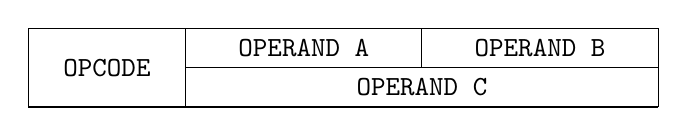
\begin{tikzpicture}
    \draw (0,0) -- (8,0);
    \draw (0,1) -- (8,1);
    \draw (2,0.5) -- (8,0.5);
    \foreach \x in {0,2,8}
        \draw (\x,0) -- (\x,1);
    \draw (5, 0.5) -- (5, 1);
    \node at (1,0.5) {\texttt{OPCODE}};
    \node at (5, 0.25) {\texttt{OPERAND C}};
    \node at (3.5, 0.75) {\texttt{OPERAND A}};
    \node at (6.5, 0.75) {\texttt{OPERAND B}};
\end{tikzpicture}
\caption{Graphic showing the two possible make ups of an instruction.}
\end{figure}

The instruction set used by the emulator consists of mathematical operations, logical operations, flow control and data management.

\begin{table}[H]
\centering
\caption{Opcodes and their meanings.}
\begin{tabular}{lll}
Code & Abbreviation & Description \\
\hline
\multicolumn{3}{l}{Mathematical Operations} \\
\texttt{0x0} & \texttt{ADD} & Add Operand A or B \\
\texttt{0x1} & \texttt{SUB} & Subtract Operand A from B \\
\hline
\multicolumn{3}{l}{Logical Operations} \\
\texttt{0x2} & \texttt{AND} & Bitwise AND of A and B \\
\texttt{0x3} & \texttt{OR}  & Bitwise OR of A and B \\
\texttt{0x4} & \texttt{NOT} & Bitwise NOT of A \\
\hline
\multicolumn{3}{l}{Flow Control} \\
\texttt{0x5} & \texttt{JMP} & Jump to C \\
\hline
\multicolumn{3}{l}{Data Management} \\
\texttt{0x6} & \texttt{STO} & Store the value in the accumulator in C \\
\end{tabular}
\end{table}

\section{Memory}

The memory is a generic synchronous 16-bit RAM modeled as an array of integers. It is connected directly to the Control Unit via an address bus (\verb|addr|) and to the rest of the processor by the data bus (\verb|data|).

The memory has a single control input, \verb|memory_control|, which can take four different signals:

\begin{table}[H]
\centering
\caption{Control signal names and descriptions for the ALU.}
\begin{tabular}{ll}
	Signal & Description \\
	\hline
	\texttt{MEM\_HIZ} & Don't drive the \texttt{data} bus.\\
	\texttt{MEM\_SET} & Set the memory at the \texttt{address} to the value of the \texttt{data} bus \\
	\texttt{MEM\_ENB} & Drive the \texttt{data} bus with the data stored at the \texttt{address}.\\
\end{tabular}
\end{table}

The memory is implemented in the \texttt{memory.c} and \texttt{memory.h} files. The function \texttt{updateMemory()} is called on each clock tick.

The size of allocated memory is determined by a \texttt{\#define} called \texttt{MEMORY\_SIZE}.

\subsection{Testing}

The memory is tested by setting each possible value to each cell in memory and then reading it back. This test can be found in \verb|tests/memory_test.c|.

If the operation fails then the following data is output to \texttt{stdout} for debugging.

\begin{itemize}
    \item The address being written to or read from
    \item The data being written or read
    \item The state of \texttt{memory\_control}.
\end{itemize}

\section{Arithmetic and Logic Unit}

The ALU module takes two inputs, A and B, and produces an output based on a control signal \verb|alu_control|.

In an effort to later simplify the control unit, the ALU's control input is just the opcode of the instruction, avoiding the need for a look-up-table. An additional signal \verb|ALU_HIZ| is required to tell the ALU not to drive the data bus when it is not being used.

The ALU is implemented in the \texttt{alu.c} and \texttt{alu.h} files. The function \texttt{updateALU()} is called on each clock tick. It consists of a single switch case that switches on the \texttt{alu\_control} input. The data bus is then driven with the output based on the inputs. Input buffering is handled by the control unit.

\subsection{Testing}

ALU testing is handled by \texttt{test/alu\_test.c}. The test cycles through each of the operations with all possible inputs, then asserts that the output on the data bus is correct. If an output is not correct then the following debugging data is printed to \texttt{stdout}: 

\begin{itemize}
    \item The type of operation
    \item The two inputs 
    \item The output
\end{itemize}

\section{Control Unit}

The control unit (CU) consists of registers and a state machine to control the flow of data through the CPU.

There are five registers in total. The \verb|program_counter| and \verb|instruction register| are used to control the CU itself, while the \verb|accumulator| and \verb|alu_buffer|s are used to store information for use in the ALU.

\begin{table}[H]
\centering
\caption{A description of the purpose of each register in the control unit.}
\begin{tabular}{ll}
    Register & Description \\
    \hline
    \verb|program_counter| & Stores the address of the current instruction. \\
    \verb|instruction_register| & Stores the current instruction being executed. \\
    \verb|accumulator| & Used to store the output of the ALU. \\
    \verb|alu_buffer_a| & Buffer for input A of the ALU. \\
    \verb|alu_buffer_b| & Buffer for input B of the ALU. \\
\end{tabular}
\end{table}

Every instruction follows a basic flow through the control unit, however the specifics vary between opcodes. The basic flow follows these five steps:

\begin{enumerate}
    \item The CU gets the next instruction from memory, based on the value of the program counter, and puts that into the instruction register. 
    \item The instruction register's value is bit shifted and pruned in order to provide the CU with values for the Opcode and Operands A, B and C.
    \item The Opcode is then used to determine the sequence though which the CU must progress.
    \item Any execution is performed.
    \item The program counter is incremented and the process begins again.
\end{enumerate}

More specifically, the CU follows the following state transition table. The system only depends on the Opcode input.

\begin{table}[H]
\centering
\caption{States and descriptions for the Control Unit State Machine.}
\begin{tabular}{p{0.2\textwidth} p{0.5\textwidth} p{0.2\textwidth}}
    State[:Opcode] & Description & Next State \\
    \hline\hline
    \verb|DECODE| & Decode the opcode and decide which state transition to go though. \\
    \verb|DECODE:JMP| & Set the program counter to operand C. & \verb|GET_INSTRUCTION| \\
    \verb|DECODE:STO| & Store the value of the accumulator at address of operand C. & \verb|INC_COUNTER| \\
    \verb|DECODE:ADD| & \multirow{5}{*}{Get the value of operand A from memory.} & \multirow{5}{*}{\texttt{ALU\_SETAGETB}} \\
    \verb|DECODE:SUB| &  & \\
    \verb|DECODE:AND| &  & \\
    \verb|DECODE:OR| &  & \\
    \verb|DECODE:NOT| &  & \\
    \hline
    \verb|ALU_SETAGETB| & Set the value of operand A from the data bus and get operand B from memory. & \verb|ALU_SETBEXEC| \\
    \hline
    \verb|ALU_SETBEXEC| & Set the value of operand B and start the exitution of the calculation in the ALU. & \verb|INC_COUNTER| \\
    \hline
    \verb|INC_COUNTER| & Set the accumulator and incriment the program counter. & \verb|GET_INSTRUCTION| \\
    \hline
    \verb|GET_INSTRUCTION| & Get the next instruction from memory. & \verb|SET_INSTRUCTION| \\
    \hline
    \verb|SET_INSTRUCTION| & Set the instruction register. & \verb|DECODE| \\
\end{tabular}
\end{table}

The CU must be initialized before any computation can take place. The initial state is described in the following table, note that any registers or states not mentioned do not require initialization.

\begin{table}[H]
\centering
\caption{The required initial state of the Control Unit to ensure proper operation of the emulator.}
\begin{tabular}{ll}
    \verb|next_state| & \verb|GET_INSTRUCTION| \\
    \verb|program_counter| & \verb|0x0000|
\end{tabular}
\end{table}

The CU is implemented in the \verb|control_unit.c| and \verb|control_unit.h| files.

With the control unit finished, the whole of the emulation code is ready. In order to properly test the control unit, a wrapper is required to load programs into memory and show outputs.

\section{Wrapper}

\section{Assembler}

\end{document}